\section{Visual exploration}

\begin{frame}[fragile]{Goals of \texttt{explore.py}}
  After a successful \texttt{bumpy.py} run, plot
  \begin{itemize}
    \item $u(t)$ and $u'(t)$ for $t \ge t_s$
    \item FFT spectra of $u$ and $F$ (dominant frequencies)
    \item stacked panels of $h(x)$, $F(t)$, and $u(t)$
          for each road realization
  \end{itemize}
\begin{lstlisting}[style=terminal]
uv run python explore.py 180
\end{lstlisting}
\end{frame}

\begin{frame}[fragile]{Loading pickled data}
  \lstinputlisting[style=pythoncompact]{code/explore_load.py}
  Boolean mask \texttt{t >= t\_s} selects the late-time window.
\end{frame}

\begin{frame}{Late-time displacement}
  \begin{center}
    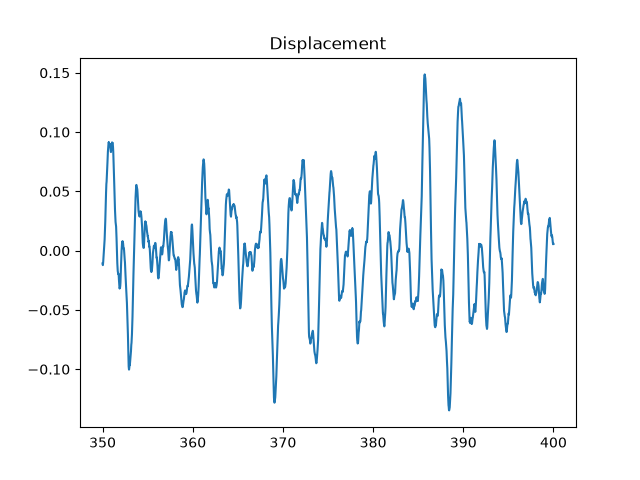
\includegraphics[width=0.72\textwidth]{figures/u1.png}
  \end{center}
\end{frame}

\begin{frame}{Velocity by centered differences}
  \[
  v^n = (u')^n \approx
  \frac{u^{n+1} - u^{n-1}}{2\Delta t}
  \quad (1\le n \le N-1),
  \]
  with one-sided formulas at the ends.
  Vectorized NumPy slicing is much faster than a Python loop.
\end{frame}

\begin{frame}{Velocity plots}
  \begin{columns}[T]
    \begin{column}{0.48\textwidth}
      \centering
      Raw\\
      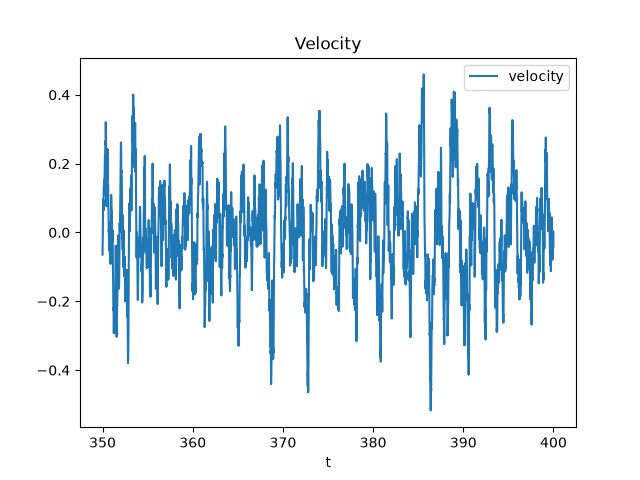
\includegraphics[width=\textwidth]{figures/v1.png}
    \end{column}
    \begin{column}{0.48\textwidth}
      \centering
      Smoothed\\
      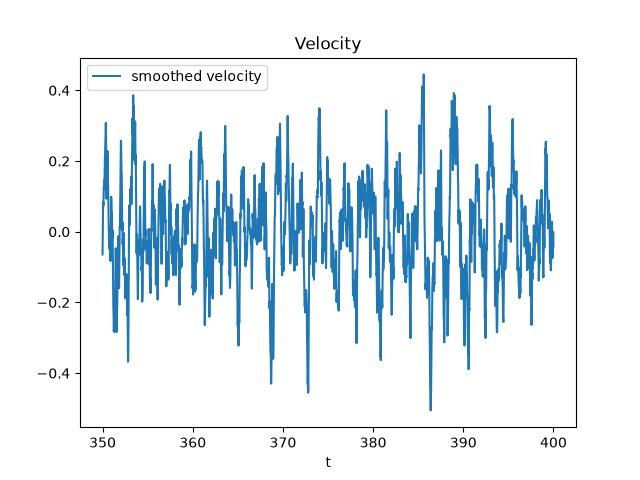
\includegraphics[width=\textwidth]{figures/v1s.png}
    \end{column}
  \end{columns}
\end{frame}

\begin{frame}[fragile]{Frequency analysis (FFT)}
  \lstinputlisting[style=pythonTiny]{code/frequency_analysis.py}
\end{frame}

\begin{frame}{Spectra}
  \begin{center}
    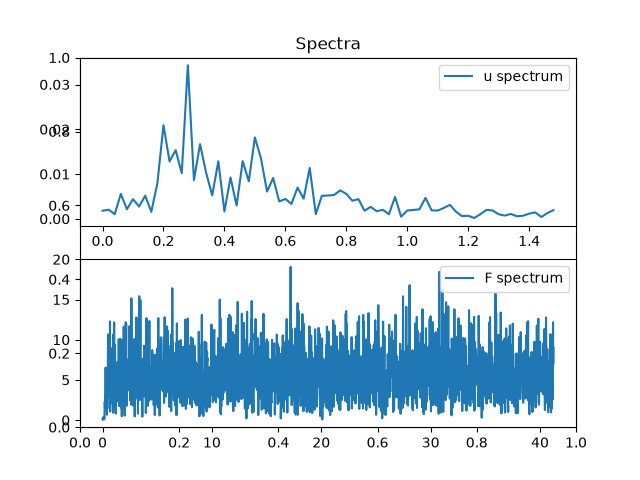
\includegraphics[width=0.68\textwidth]{figures/spectra1.png}
  \end{center}
\end{frame}

\begin{frame}{Road, force, and displacement}
  \begin{center}
    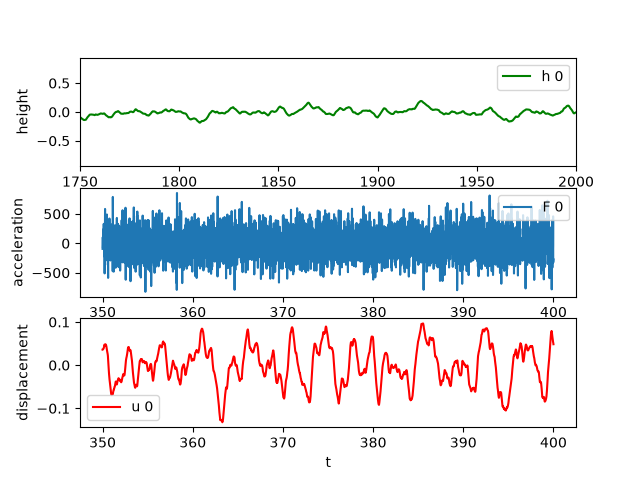
\includegraphics[width=0.62\textwidth]{figures/hFu0.png}
  \end{center}
\end{frame}

\begin{frame}[fragile]{Animation options}
\begin{lstlisting}[style=terminal]
uv run python bumpy_road_anim.py --help
uv run python bumpy_road_anim.py --frames 60 --fps 10
uv run python bumpy_road_anim.py --roadfile draw_bumpy.csv
uv run python bumpy_road_anim.py --roadfile bumpy.csv --profile 0
\end{lstlisting}
  Default road is a built-in sine profile; CSV roads are interpolated.
\end{frame}
